% === Begin Label Data ===
% ID: 753
% 难度星级: 
% 标签: 
% 备注: 
% 组卷引用次数: 0
% === End  Label Data ===

\begin{problem}{2014}{G}{安徽卷（理）}{10}{向量}
在平面直角坐标系 $ xOy $ 中，已知向量 $ \vec{a},\vec{b},|\vec{a}|=|\vec{b}|=1,\vec{a}\cdot\vec{b}=0 $，点 $ Q $ 满足 $ \overrightarrow{OQ}=\sqrt{2}(\vec{a}+\vec{b}) $．曲线 $ C=\left\{P\middle|\overrightarrow{OP}=\vec{a}\cos\theta+\vec{b}\sin\theta,0\leqslant\theta<2\pi\right\} $，区域 $ \Omega=\left\{P\middle|0<r\leqslant|PQ|\leqslant R,r<R\right\} $．若 $ C\cap\Omega $ 为两段分离的曲线，则 (\hspace{1cm})
\begin{choices}
\choice{{$1<r<R<3$}}
\choice{{$1<r<3\leqslant R$}}
\choice{{$r\leqslant1< R<3$}}
\choice{{$1<r<3<R$}}
\end{choices}
\end{problem}

\begin{answer}
$ A $
\end{answer}

\begin{solutions}
不妨设 $ \vec{a}=(1,0),\vec{b}=(0,1),\overrightarrow{OQ}=(\sqrt{2},\sqrt{2})\Rightarrow|\overrightarrow{OQ}|=2 $．

$ \overrightarrow{OP}=(\cos\theta,\sin\theta) $，曲线 $ C $ 即是圆 $ O:x^{2}+y^{2}=1 $．

区域 $ \Omega $ 是一个以 $ P $ 为圆心的圆环，画出临界状态：

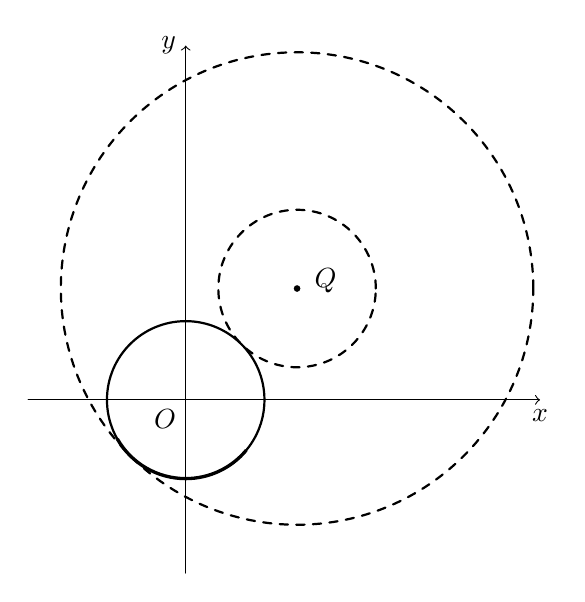
\begin{tikzpicture}[line cap=round,line join=round,scale=1]
\usetikzlibrary{calc}

% axes
\draw[->] (-2.0,0) -- (4.5,0) node[below] {$x$};
\draw[->] (0,-2.2) -- (0,4.5) node[left] {$y$};

% key points
\coordinate (O) at (0,0);
\coordinate (Q) at ({sqrt(2)},{sqrt(2)});

\node[below left] at (O) {$O$};
\fill (Q) circle (1.2pt);
\node[right] at ($(Q)+(0.1,0.1)$) {$Q$};

% circle C: x^2 + y^2 = 1
\draw[thick] (O) circle (1);

% annulus boundaries centered at Q: radii 1 and 3 (dashed)
\draw[dashed,thick] (Q) circle (1);
\draw[dashed,thick] (Q) circle (3);

% small arc highlight on circle C (schematic, like the picture)
\draw[very thick] (O) ++(210:1) arc[start angle=210,end angle=320,radius=1];

\end{tikzpicture}


圆 $ Q $ 与圆 $ O $ 外切和内切对应的半径分别为 $ 1 $ 和 $ 3 $，

进而 $ r\leqslant1 $ 或 $ R\geqslant3 $ 时 $ C\cap\Omega $ 是完整的一段圆弧或者圆，不满足题意，于是选 $ A $．
\end{solutions}